
\noindent\begin{minipage}{\textwidth}
    \begin{table}[H]
        \centering
        \caption{Hiperparâmetros e Resultados do Melhor Modelo - vit\_v9\_AM\_opt\_aug}
        \vspace{0.2cm}
        \resizebox{\textwidth}{!}{%
            \begin{tabular}{ll | lrrr}
                \hline
                \multicolumn{2}{c|}{\textbf{Hiperparâmetros}} & \multicolumn{4}{c}{\textbf{Métricas por Classe}} \\ \hline
                \textbf{Parâmetro} & \textbf{Valor} & \textbf{Classe} & \textbf{Precisão} & \textbf{Recall} & \textbf{F1-Score} \\ \hline
    Agendador (Patience) & 8 & 31.2 & 0,5775 & 0,4779 & 0,5230 \\ 
Agendador de LR & ReduceLROnPlateau & 31.3 & 0,3431 & 0,4653 & 0,3950 \\ 
Architecture & vit\_b\_16 & 31.4 & 0,3333 & 0,4048 & 0,3656 \\ 
Augmentation (Método) & None & 32.3 & 0,5351 & 0,6224 & 0,5755 \\ 
Batch Size & 32 & 32.4 & 0,3913 & 0,1552 & 0,2222 \\ 
Decaimento de Peso (WD) & 0,0215 & 33.3 & 0,5590 & 0,4663 & 0,5085 \\ 
Dropout & 0,0588 & 41.4 & 0,3438 & 0,2500 & 0,2895 \\ 
Função de Perda & CrossEntropyLoss & 41.5 & 0,5510 & 0,6923 & 0,6136 \\ 
Hidden Units & 256 & 42.4 & 0,6452 & 0,2941 & 0,4040 \\ 
Label Smoothing & 0,0392 & 44.4 & 0,6800 & 0,5862 & 0,6296 \\ 
\cline{3-6} 
Otimizador & AdamW & \textbf{Média (Macro)} & 0,4994 & 0,4821 & 0,4790 \\ 
Taxa de Aprendizado (LR) & 1,59e-05 & \textbf{MCC} & \multicolumn{3}{c}{0,4059} \\ 
Unfreeze Layers & 4 &  & & &  \\ 
            \hline
            \end{tabular}%
        }
    \end{table}

    \begin{figure}[H]
        \centering
        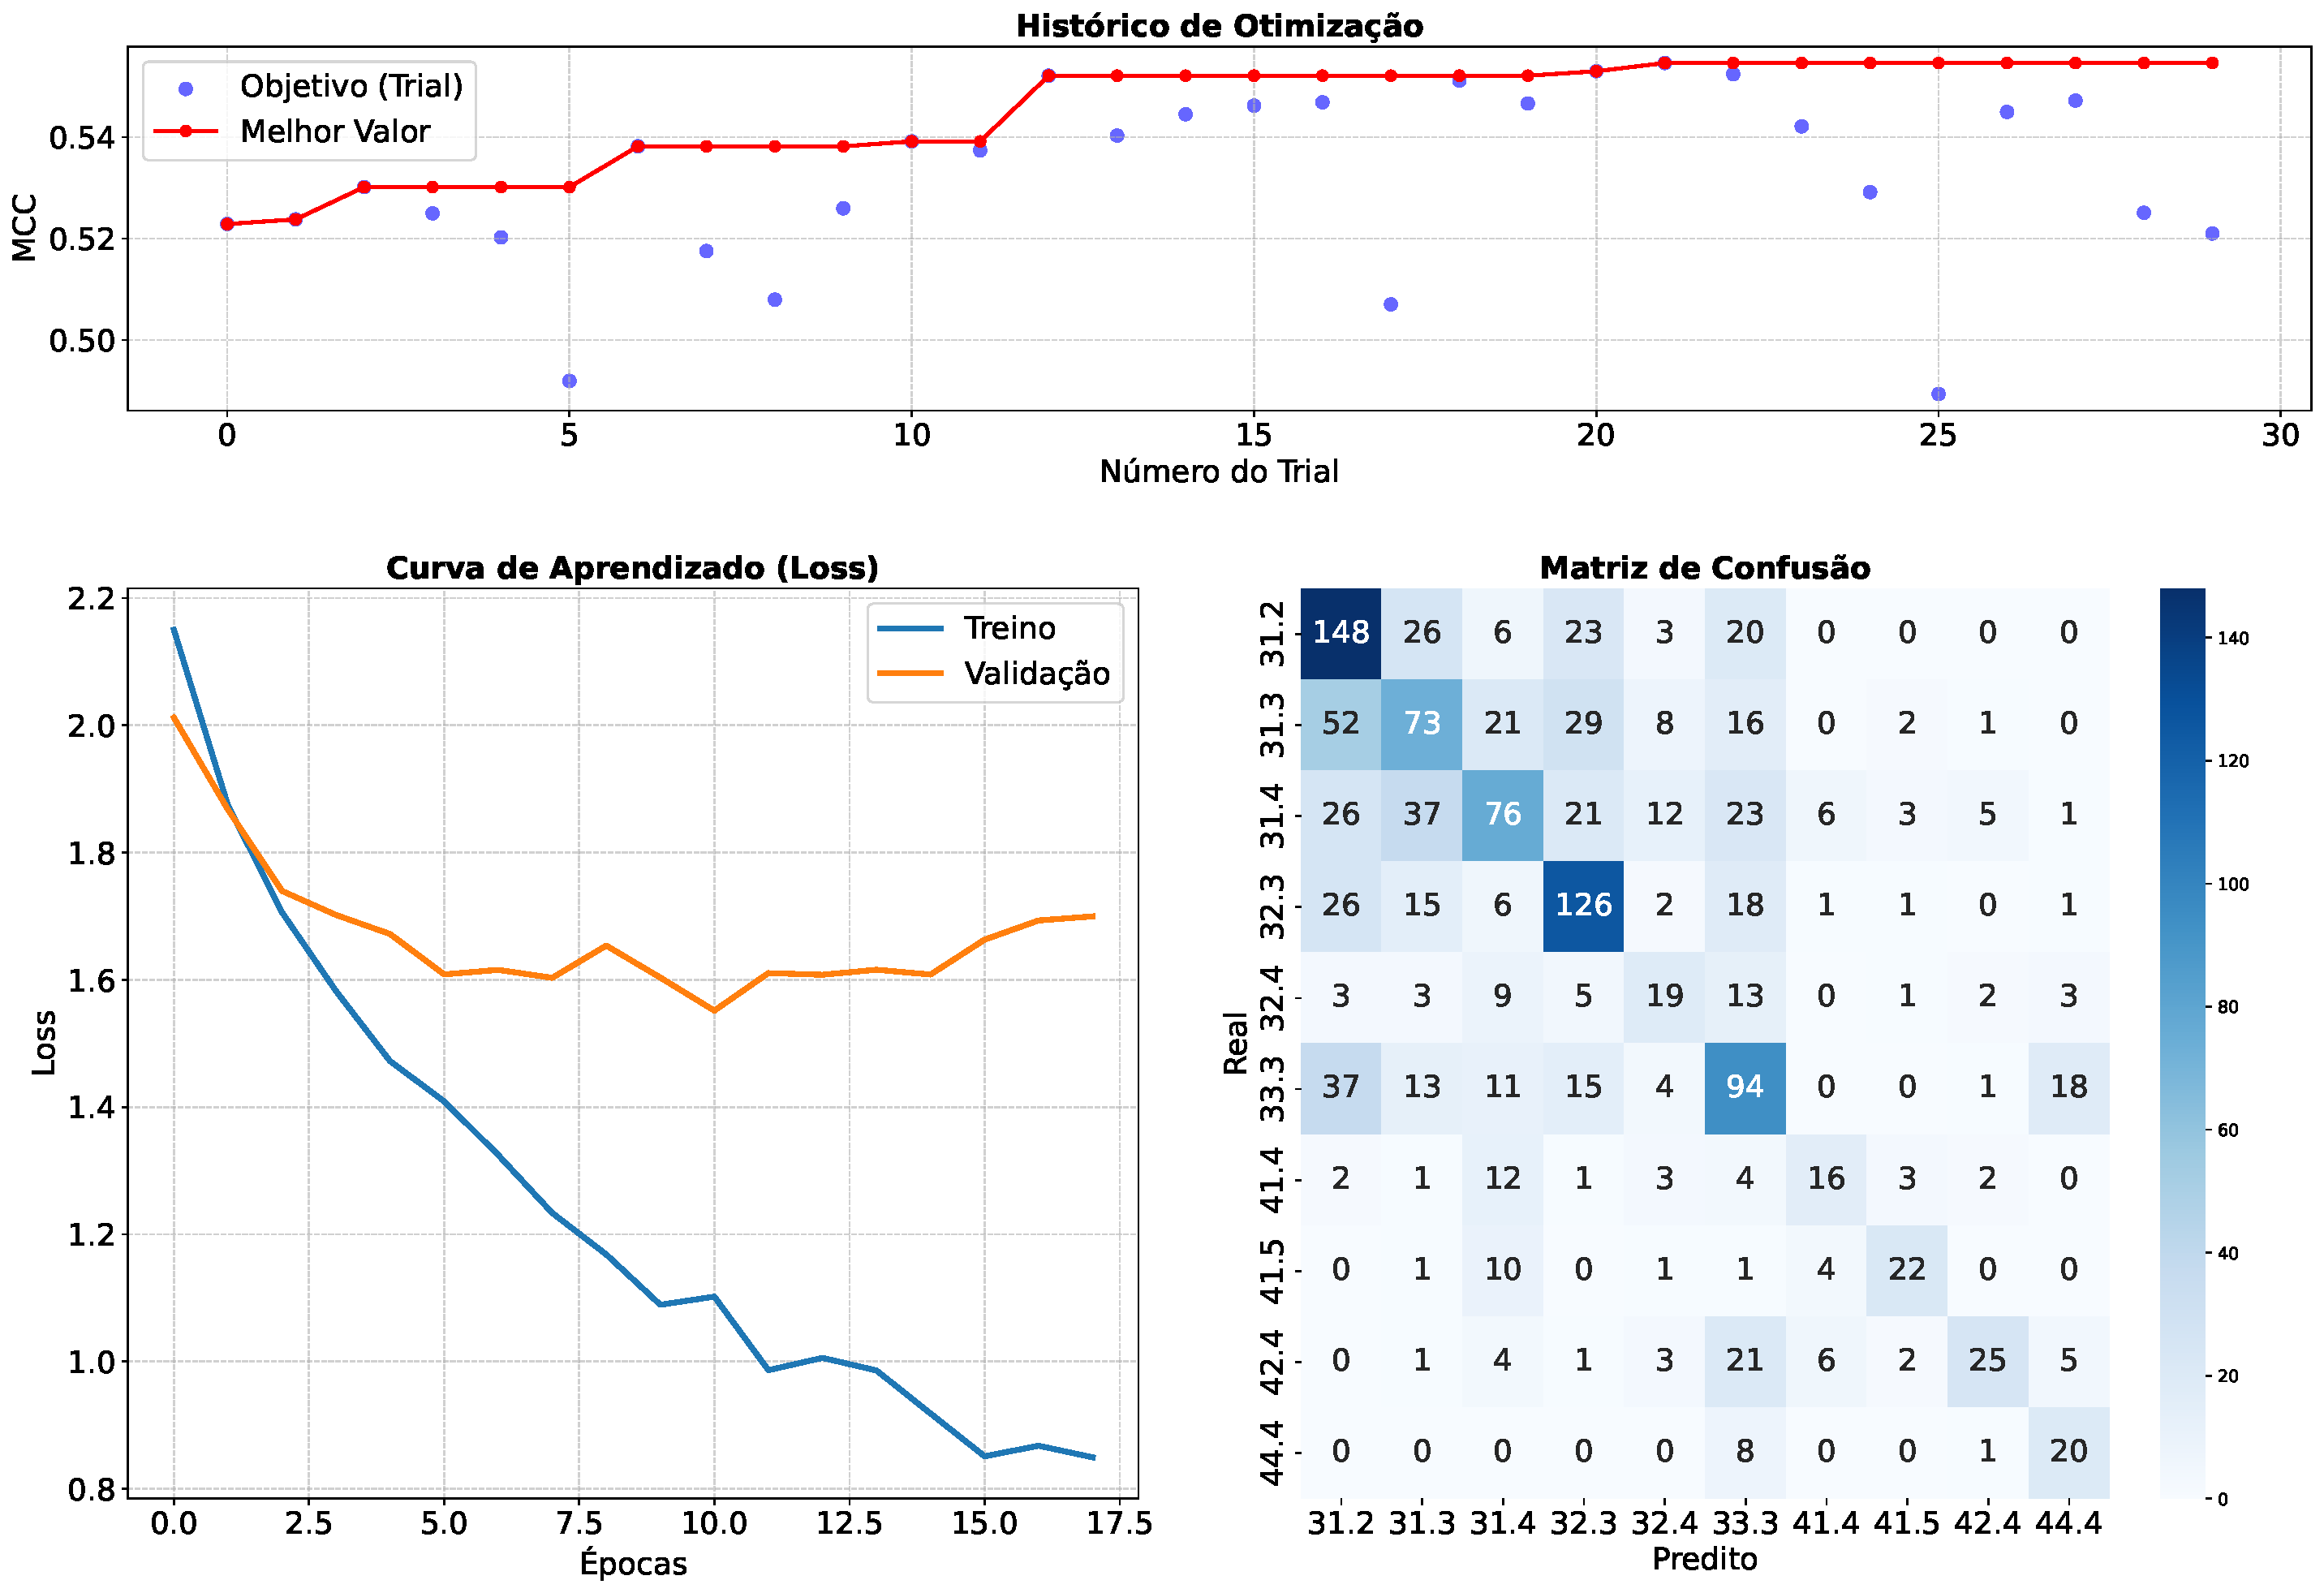
\includegraphics[width=0.85\textwidth]{tex/appendix/experiments/vit_v9_AM_opt_aug/dashboard_consolidado.pdf}
        \caption{Histórico de Otimização, Curvas de Aprendizado e Matriz de Confusão - vit\_v9\_AM\_opt\_aug}
    \end{figure}
\end{minipage}
\clearpage
